% Generated from ../chapters/03-causation-across-levels.md
\chapter{Causation Across Levels}\label{chapter-3-causation-across-levels}

Complex systems are organized in levels. In a human society, individuals form teams, institutions, markets, and cultures. In a body, molecules form organelles, cells, tissues, organs, physiological systems, behavior, and a person embedded in a social world. Each level is made from lower-level components, but it also changes the conditions under which those components act.

Reductionism proceeds downward. To understand a fever, examine cytokines, immune cells, receptors, and pathogens. To understand muscle contraction, examine actin, myosin, calcium, and ATP. This strategy has been spectacularly successful because higher-level events must be physically implemented.

The mistake is to infer that implementation makes the lower level the only real cause.

Consider a company. A decision by its board may cause thousands of computers to run different software the next morning. Nothing supernatural occurred. The decision was implemented through emails, contracts, access controls, managers, and keyboards. Yet explaining every electron in the computers would not reveal why the change happened. The organizational decision altered boundary conditions for lower-level events.

George Ellis calls such effects \textbf{top-down causation}: higher-level structures select, constrain, or enable lower-level processes \autocite{ellis2012topdown}. Denis Noble's principle of \textbf{biological relativity} makes a related point: biology has no universally privileged level of causation \autocite{noble2012biological}. A gene can influence behavior, and behavior can influence gene expression. The causal arrows form loops.

In a body, a sentence such as ``I will train for a marathon'' can become biological. The sentence is not a molecule. It is a high-level commitment. It changes a calendar, sleep, food, social relations, attention, repeated motor output, endocrine signals, blood flow, mechanical loading, and gene expression. The commitment reaches cells because the person reorganizes the conditions in which those cells live.

This is downward causation without mysticism. Beliefs do not violate physics. They are patterns instantiated in nervous systems and social relations that constrain what physical actions occur next.

The same logic operates in the opposite direction. An inflammatory signal alters mood. Sleep loss changes judgment. Pain changes identity. Causation is circular because levels continually modify one another.

\begin{figure}
\centering
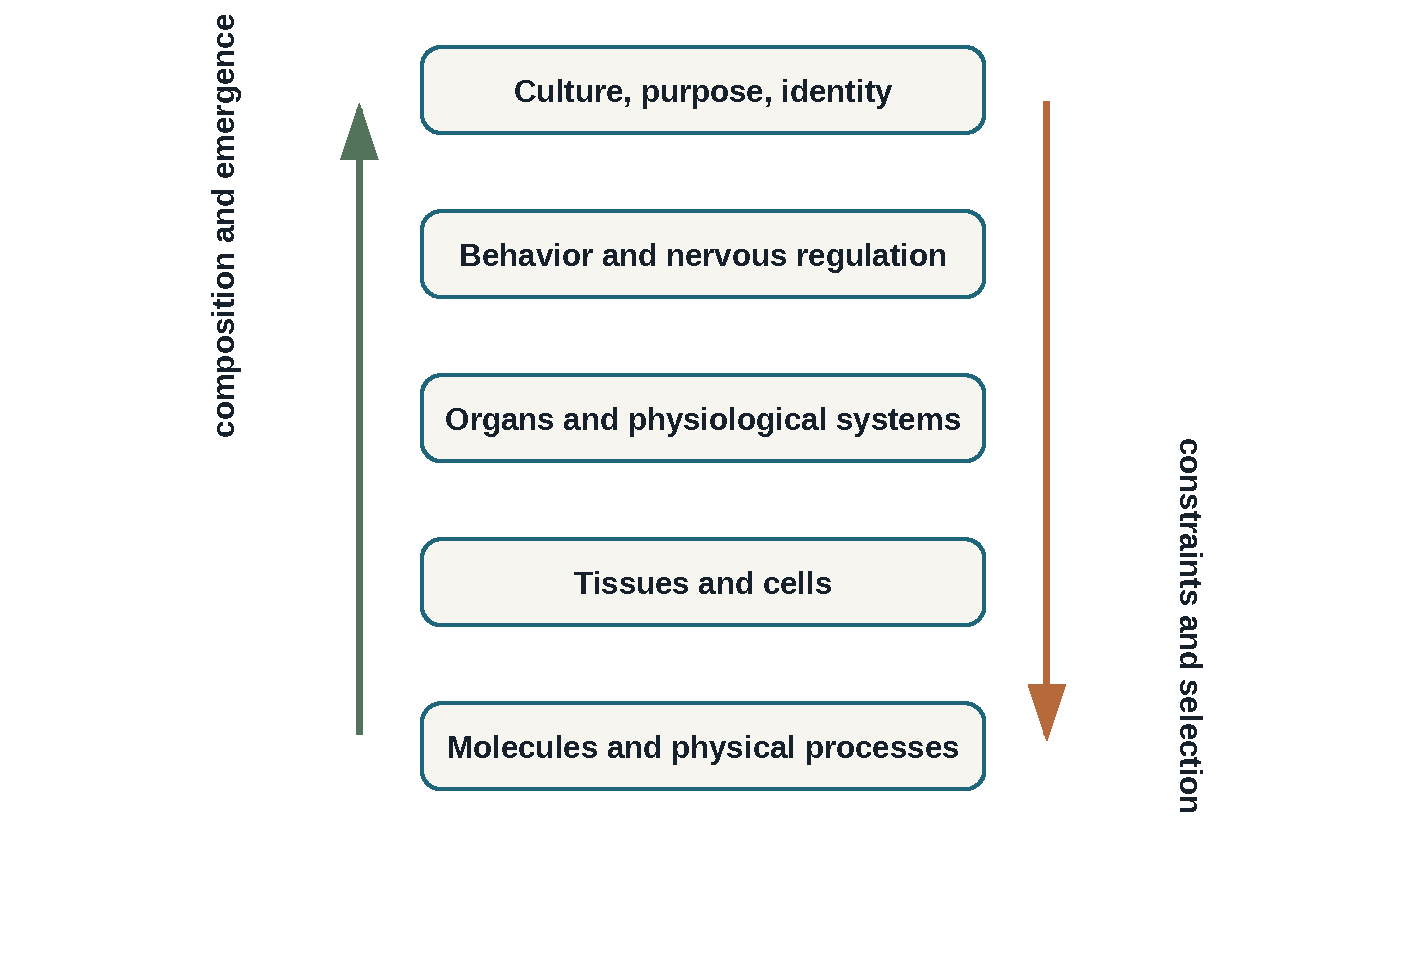
\includegraphics[width=0.82\textwidth,height=.68\textheight]{../figures/causal-hierarchy.pdf}
\caption{Causal influence moves upward through composition and downward through constraints. No single level is sufficient for a complete explanation.}\label{fig:hierarchy}
\end{figure}

The concept becomes useful when it prevents two errors. The first is molecular reductionism: assuming that only an intervention delivered as a drug or gene therapy is biologically deep. A social role, a long project, a movement practice, or an expectation can generate molecular effects through long causal chains. The second error is holistic vagueness: invoking ``mind over matter'' without specifying any pathway. A serious top-down account must identify the intermediate mechanisms.

Pain offers a concrete example. A prediction of danger can produce anticipatory bracing. Bracing alters force distribution and sensory feedback. The new sensations confirm the prediction, deepening the attractor. Safe exposure, skill, and a revised interpretation can reverse part of the loop. This does not mean all pain is psychological. It means that in systems containing perception and action, interpretation is one causal variable among others.

The broader implication is that longevity cannot be reduced to molecules alone. A person's work, identity, family, culture, and expectations shape daily behavior for decades. Their effects are diffuse and difficult to randomize, but difficulty of measurement is not evidence of causal irrelevance.
